\subsubsection{User Administration}
This package defines the logic behind the creation and the management of Users, their registrations and their logins.


\class{Registration}

\begin{figure}[H]
\centerline{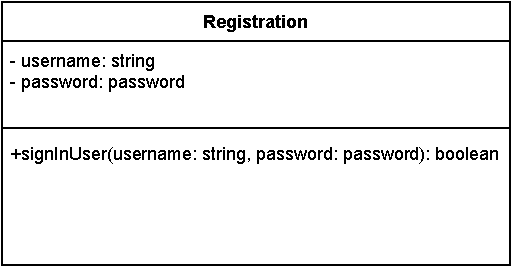
\includegraphics[scale=1]{res/Klassen/RegistrationClass.pdf}}
\caption{Registration class from class diagram}
\end{figure}

This class is used to sign up new Users for our application and also for airflow.


\begin{methodenv}{Methods}

\method{signUser(username: String, password: password): boolean}

Method uses username and password to sign up new user and returns a boolean to confirm the registration

\smallPara{Parameters}
\begin{itemize}
	\item{username:}
	The preferred username
	\item{password:}
	The preferred password
\end{itemize}

\smallPara{Exceptions}
\begin{itemize}
	\item{UserExistsException}
	Gets thrown if the user trys to register with an already used username
\end{itemize}
\end{methodenv}



\class{User}

\begin{figure}[H]
\centerline{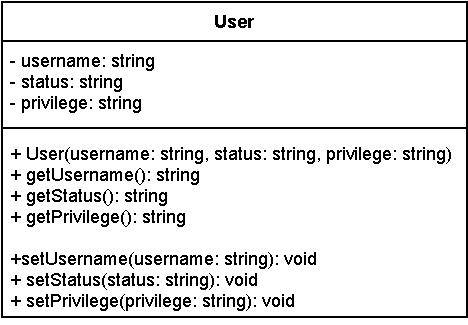
\includegraphics[scale=1]{res/Klassen/UserClass.pdf}}
\caption{User class from class diagram}
\end{figure}

This class is used to construct new Users.
\begin{methodenv}{Constructor}

\method{user(username: string, status: string, privilege: string)}

\smallPara{Parameters}

\begin{itemize}
	\item{username:}
	The users username
	\item{status:}
	The users status. Can be active, inactive or banned
	\item{privilege:}
	The users privilege. Can be Reviewer, Develloper or Admin
\end{itemize}
\end{methodenv}



\class{Login}

\begin{figure}[H]
\centerline{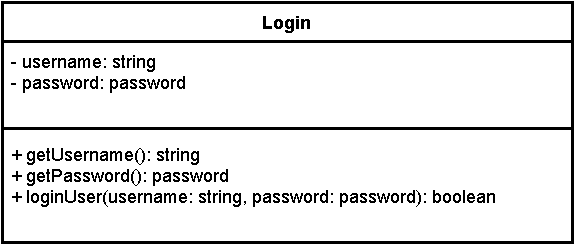
\includegraphics[scale=1]{res/Klassen/LoginClass.pdf}}
\caption{Login class from class diagram}
\end{figure}

This class is used to log in existing Users.

\begin{methodenv}{methods}

\method{loginUser(username: String, password: password): boolean}

Method uses username and password to log in user and returns a boolean to confirm the login.

\smallPara{Parameters}
\begin{itemize}
	\item{username:}
	The username to log in
	\item{password:}
	The password to log in
\end{itemize}
\end{methodenv}




\class{UserController}

\begin{figure}[H]
\centerline{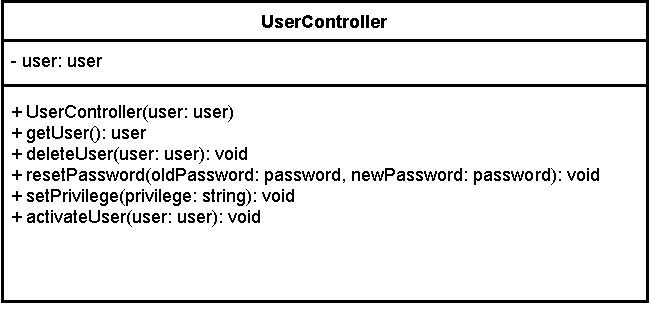
\includegraphics[scale=1]{res/Klassen/UserControllerClass.pdf}}
\caption{UserController class from class diagram}
\end{figure}

This class is used to change the parameters of existing users.

\begin{methodenv}{Constructor}

\method{UserController(user: user)}

\smallPara{Parameters}

\begin{itemize}
	\item{user:}
	The user that needs to be edited
\end{itemize}
\end{methodenv}

\begin{methodenv}{Methods}

\method{deleteUser(user:user): void}

Method gets the wanted User and deltes him. Afterwards the user is not able to log in anymore.

\smallPara{Parameters}
\begin{itemize}
	\item{user:}
	The user that is supposed to get deleted
\end{itemize}


\method{resetPassword(oldPassword: password, newPassword: password): void}

Method resets the users password and sets the new password.

\smallPara{Parameters}
\begin{itemize}
	\item{oldPassword:}
	The users old password that gets deleted
	\item{newPassword:}
	The users new password that is getting set
\end{itemize}

\method{setPrivilege(privilege: string): void}

Method resets the users old privilege and updates to the new privilege.

\smallPara{Parameters}
\begin{itemize}
	\item{privilege:}
	The privilege the user gets updated to
\end{itemize}

\method{activateUser(): void}

Method activates the User. The User can now log in to the application.

\end{methodenv}










